\chapter{Permutations of \ch{(CrFeMnNi)Si2}}
\label{sec:permutations}

Up until this point we have looked in detail at the high-entropy silicide \ch{(CrFeMnNi)Si2} and associated SQSs. However these structures are just the center of a larger quasi-ternary phase diagram consisting of the different possible distributions of elements Thus there exists many other compositions of this particular high-entropy silicide. In this section, we aim to expand our search of this diagram by generating SQSs of the 48 atom model slightly away from equimolar distribution of 3d elements. In table (bellow) we list the mean total energy and magnetic moment per atom with standard deviation and the enthalpy of formation of 4 compositions of the \ch{(CrFeMnNi)Si2} alloy. Ideally they would differ only by one element, but the TDEP implementation insist in also reducing Nickel to stay consistent with the 48 atom supercell. 

\begin{table}[H]
\centering
\begin{tabular}{@{}cccccc@{}}
\toprule
Composition           & \multicolumn{2}{c}{\begin{tabular}[c]{@{}c@{}}Toten\\ (eV)\end{tabular}} & \multicolumn{2}{c}{\begin{tabular}[c]{@{}c@{}}Mag \\ $\mu_B$\end{tabular}} & \begin{tabular}[c]{@{}c@{}}$\Delta H$\\ (eV)\end{tabular} \\ \midrule
                      & mean                                 & std                               & mean                                 & std                                 & mean                                                      \\ \midrule
\ch{Cr3Fe3Mn7Ni3Si32} & - 6.6947                             & 0.0040                            & 0.1375                               & 0.0186                              & -11.9586                                                  \\
\ch{Cr5Fe5Mn3Ni3Si32} & - 6.6705                             & 0.0030                            & 0.1127                               & 0.0223                              & -11.1991                                                  \\
\ch{Cr5Fe3Mn5Ni3Si32} & - 6.6852                             & 0.0041                            & 0.1375                               & 0.0456                              & -10.5200                                                  \\
\ch{Cr3Fe5Mn5Ni3Si32} & - 6.6801                             & 0.0036                            & 0.0937                               & 0.0209                              & -12.6426                                                  \\
\ch{Cr3Fe3Mn3Ni7Si32} & - 6.3921                             & 0.0078                            & 0.0159                               & 0.0101                              & -10.9614                                                  \\ \bottomrule
\end{tabular}
\caption{Summary composition diagram}
\end{table}

The first result of table .. we make notice of is that the stability, as evaluated by the enthalpy of formation can be increased beyond the eqvimolar composition. This is accomplished in two distinct permutations, one with increments to  manganese relative to the other TM, and the other by reduction of chromium. Moreover the two respective permutations lie on the opposite side of the magnetic scale. The large magnetic moment of the manganese rich permutation and the low magnetic moment in the chromium poor permutation is very much in line with the observations made in the previous section. Recalling that in the magnetic moment in the eqvimolar composition was largely attributed to manganese and chromium atoms in the lattice. Thus increments to manganese or reduction of chromium would following impact the magnetic moment as in the two permutations. For this reason, additionally the permutation \ch{Cr5Fe3Mn5Ni3Si32} where the nonmagnetic elements is reduced and the magnetic elements are increased ,is equally magnetic. We however find no direct relation between stability and magnetism as his particular permutation is the least stable. An important property of table 8.5 is that the listed values are the mean value of the observed property for 5 distinct SQSs of the same permutation. For example we notice that while the highest magnetic moment in the first permutation is associated with the most stable SQS (from total energy considerations), and the least stable supercell show the highest magnetic moment in \ch{Cr5Fe3Mn5Ni3Si32}. Hence again we find the uniqeness problem of the special quasi-random structures troublesome in regards to making rigid conclusions of our results.  

In table 8.2 we list the respective band gaps of the different compositions calculated with the PBE functional. Only the GGA functional was applied in this case because the motivation is primarily to compare the results to the parent equimolar composition and thus including 3 times as many results to calculate and analyze unnecessarily complicate the process. Thus we base this comparison between the PBE results of the new compositions to the PBE band gaps of the equimolar compound. In these compositions we find strong indication of a half-metal with less frequent SQSs with a band gap in the spin down channel than the equimolar compound. In the spin up channel on the other hand several compositions show very similar values to the equimolar composition. Between the different compositions particularly those rich in manganese provide very encouraging results and compositions poor in Mn less so. In terms of the stability we a very encouraging results of both the \ch{Cr3Fe3Mn7Ni3Si32} and \ch{Cr3Fe5Mn5Ni3Si32} compositions, where the most promising properties is attributed to the utmost stable configurations.  in \ch{Cr3Fe5Mn5Ni3Si32} the most stable SQS (D) is a semiconductor with a band gap around 0.1 eV.

\newpage
% Please add the following required packages to your document preamble:
% \usepackage{booktabs}
% \usepackage{multirow}
\begin{table}[]
\begin{tabular}{@{}ccccc@{}}
\toprule
Composition                                                 & SQS        & \begin{tabular}[c]{@{}c@{}}$E_G ^\text{up, eigen}(0.5)$\\ (eV)\end{tabular} & \begin{tabular}[c]{@{}c@{}}$E_G ^\text{dw, eigen}(0.5)$\\ (eV)\end{tabular} & \begin{tabular}[c]{@{}c@{}}$E_G ^\text{tot, eigen}(0.5, 0.5)$\\ (eV)\end{tabular} \\ \midrule
\multicolumn{1}{c|}{\multirow{5}{*}{\ch{Cr3Fe3Mn7Ni3Si32}}} & A          & 0.3390                                                                      & 0                                                                           & 0                                                                                 \\
\multicolumn{1}{c|}{}                                       & \textbf{B} & 0.4745                                                                      & 0                                                                           & 0                                                                                 \\
\multicolumn{1}{c|}{}                                       & C          & 0.1342                                                                      & 0                                                                           & 0                                                                                 \\
\multicolumn{1}{c|}{}                                       & D          & 0.1950                                                                      & 0.0063                                                                      & 0.0063                                                                            \\
\multicolumn{1}{c|}{}                                       & E          & 0.4211                                                                      & 0                                                                           & 0                                                                                 \\ \midrule
\multicolumn{1}{c|}{\multirow{4}{*}{\ch{Cr5Fe5Mn3Ni3Si32}}} & A          & \textit{0.003}                                                              & 0                                                                           & 0                                                                                 \\
\multicolumn{1}{c|}{}                                       & \textbf{C} & \textit{0.21}                                                               & 0                                                                           & 0                                                                                 \\
\multicolumn{1}{c|}{}                                       & D          & 0.0674                                                                      & 0.0413                                                                      & 0.0372                                                                            \\
\multicolumn{1}{c|}{}                                       & E          & \textit{0.362}                                                              & 0                                                                           & 0                                                                                 \\ \midrule
\multicolumn{1}{c|}{\multirow{5}{*}{\ch{Cr5Fe3Mn5Ni3Si32}}} & \textbf{A} & 0.2082                                                                      & 0                                                                           & 0                                                                                 \\
\multicolumn{1}{c|}{}                                       & B          & 0.4053                                                                      & 0                                                                           & 0                                                                                 \\
\multicolumn{1}{c|}{}                                       & C          & 0.4659                                                                      & 0                                                                           & 0                                                                                 \\
\multicolumn{1}{c|}{}                                       & D          & 0.0843                                                                      & 0.0121                                                                      & 0.0121                                                                            \\
\multicolumn{1}{c|}{}                                       & E          & 0.3008                                                                      & 0                                                                           & 0                                                                                 \\ \midrule
\multicolumn{1}{c|}{\multirow{4}{*}{\ch{Cr3Fe5Mn5Ni3Si32}}} & A          & 0.3922                                                                      & 0                                                                           & 0                                                                                 \\
\multicolumn{1}{c|}{}                                       & C          & 0.1285                                                                      & 0                                                                           & 0                                                                                 \\
\multicolumn{1}{c|}{}                                       & \textbf{D} & 0.2595                                                                      & 0.1004                                                                      & 0.1004                                                                            \\
\multicolumn{1}{c|}{}                                       & E          & 0.3591                                                                      & 0.1003                                                                      & 0.0848                                                                            \\ \midrule
\multicolumn{1}{c|}{\multirow{5}{*}{{Cr3Fe3Mn3Ni7Si32}}}    & A          & 0                                                                           & 0                                                                           & 0                                                                                 \\
\multicolumn{1}{c|}{}                                       & B          & 0                                                                           & 0                                                                           & 0                                                                                 \\
\multicolumn{1}{c|}{}                                       & C          & 0                                                                           & 0                                                                           & 0                                                                                 \\
\multicolumn{1}{c|}{}                                       & D          & 0                                                                           & 0                                                                           & 0                                                                                 \\
\multicolumn{1}{c|}{}                                       & \textbf{E} & \textit{0.04}                                                               & 0                                                                           & 0                                                                                 \\ \bottomrule 
\end{tabular}

\caption{Band gaps of various compositions of \ch{(CrFeMnNi)Si2}. Most stable SQS of a set is highlighted in bold text, band gap with defect states are listed in cursive. Some SQSs were excluded from the table due to unsuccessful calculations.}
\end{table}
\newpage

Below in figure 8.1 we plot the projected density of states around $E_F$ of the fist four compositions of table 8.2. Note that away from the Fermi energy the projected density of states is analogous to the parent equimolar composition. The below figures is based on the most stable SQS in each permutation, as will the analysis. Hence the features of these figures can be subject to the uniqueness of that particular SQS rather than a distinct feature of the exact composition, but as stated previously the most stable configuration provide the most likely properties of the composition within the scope of this project. 

\begin{figure}[H]
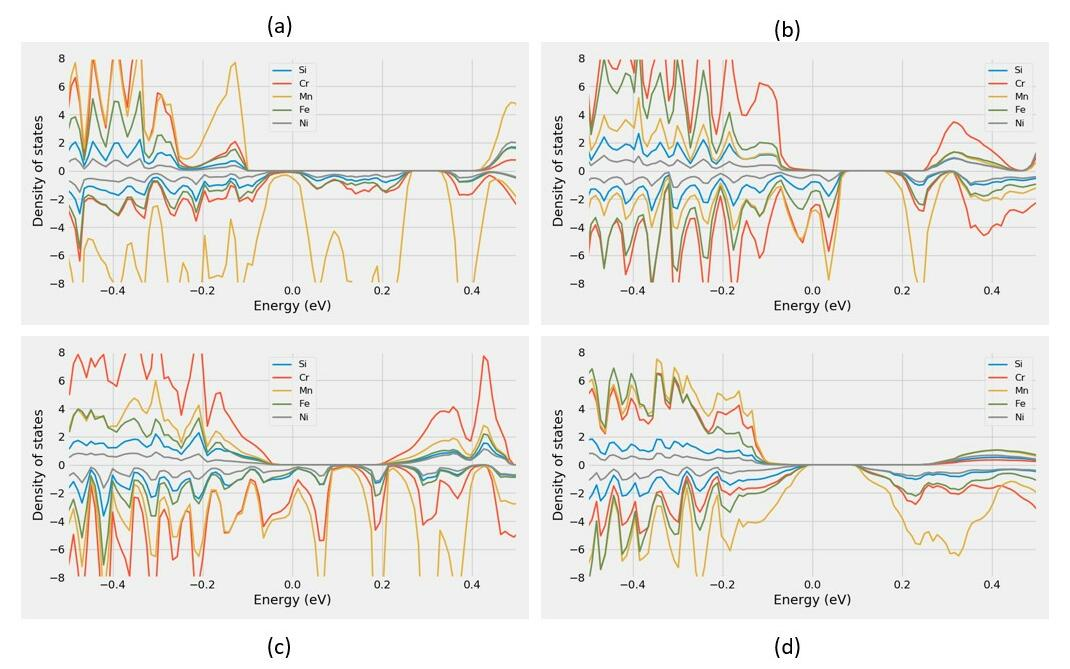
\includegraphics[width=\linewidth]{results/fesi2/permutations/perm_LDOS_crop.jpg}
\caption{Projected density of states of (a) \ch{Cr3Fe3Mn7Ni3Si32} (SQS B), (b) \ch{Cr5Fe5Mn3Ni3Si32} (SQS C), (c) \ch{Cr5Fe3Mn5Ni3Si32} (SQS A), (d) \ch{Cr3Fe5Mn5Ni3Si32} (SQS D)}
\end{figure}

With that said, the plotted PDOSs in figure 7.1 is in good agreement with the listed values in table 7.2. \ch{Cr3Fe3Mn7Ni3Si32} (7.1 a) and \ch{Cr5Fe3Mn5Ni3Si32} (7.1 c) both indicate a sizable spin up band gap, further figure (7.1 d) point to a total band gap around 0.1 eV for SQS D of \ch{Cr3Fe5Mn5Ni3Si32}. On the other hand we find dissimilarity between the density of \ch{Cr5Fe5Mn3Ni3Si32} SQS C and the eigenvalue band gap listed in table 7.2. In figure 7.1 d we find a range of forbidden energies slightly above the Fermi energy, and very small values in spin up at the Fermi energy. Similar to what we experienced in the 192 atom SQS in section 7.4, the eigenvalues report a finite band despite of defect states. Therefore the density of states is not completely zero at $E_F$. 

\begin{figure}[H]
	\centering
	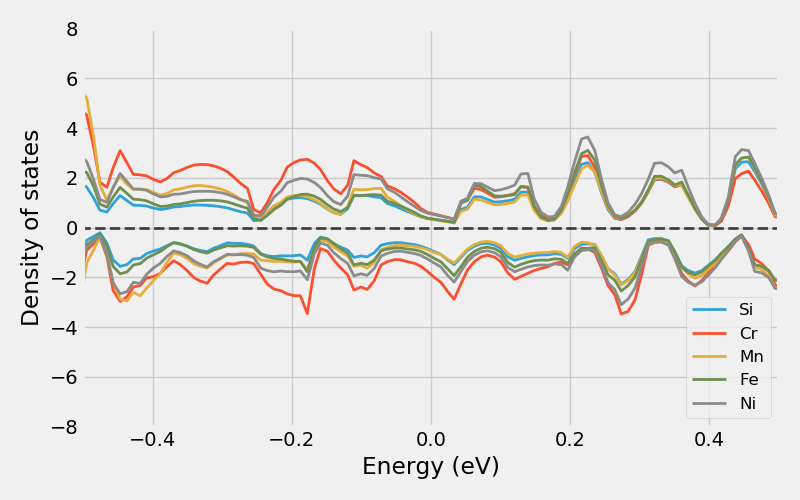
\includegraphics[width=.8\textwidth]{results/fesi2/permutations/ni7_PDOS.png}
	\caption{Projected density of states of \ch{Cr3Fe3Mn3Ni7Si32} around $E_F$}
\end{figure}

In figure 8.6 we saw that electrons from manganese atoms in particular was a key contributor as to why the spin down channel of \ch{(CrFeMnNi)Si2} was metallic in the stable supercell D. This is also largely the case in the permutations shown above in figure 8.12. The proportion of manganese atoms in the alloy seems to offer a very positive effect on the band gap in spin up, but is often detrimental to spin down. This is seen in figure 8.12 (a) and (c) for \ch{Cr3Fe3Mn7Ni3Si32} and \ch{Cr5Fe3Mn5Ni3Si32} respectively, that both contain increased amounts of manganese. By reducing the number of Mn as in (b) we still find that the Mn electrons plague the states at $E_F$ in spin down. In analog we see from (b) and (c) that also Cr negatively impacts to the band gap especially in spin up. The sole permutation with clear evidence of a spin down gap is from the chromium poor permutation plotted in (d). Also in this structure we see that the effects of Mn around $E_F$ is dampened in comparison to the other permutations, despite containing relatively increased amounts of Mn to the eqvimolar alloy.  

An important property of these results is that because each permutation alters simultaneous elements, interpreting and relating the results to a particular alteration is challenging. For example, is the result of the \ch{Cr5Fe3Mn5Ni3Si32} permutation a consequence of less Fe or increments to both Cr and Mn? Furthermore is the large band gap in spin up of \ch{Cr3Fe3Mn7Ni3Si32} a product of increasing manganese or reducing the other elements. From the comparatively large gaps in spin up of \ch{Cr3Fe3Mn7Ni3Si32} and \ch{Cr3Fe5Mn5Ni3Si32} and the more present Cr states in spin up in the Cr rich permutations we here conclude that the band gap is related to lessening of chromium, more so than other effects. However we see from both \ch{Cr5Fe5Mn4Ni3Si32} and \ch{Cr3Fe3Mn3Ni7Si32} (figure 8.2) in addition to the manganese rich composition that Mn plays a vital role on the band gap of these structures. It's clear that the \ch{Cr3Fe5Mn5Ni3Si32} alloy manage to strike a balance between 3d elements that results in a specific interplay and correspondingly very promising properties. 

